\documentclass[10pt,a4paper]{article}
\usepackage[utf8]{inputenc}
\usepackage[francais]{babel}
\usepackage[T1]{fontenc}
\usepackage{hyperref}
\usepackage{eurosym}
\usepackage{ amssymb }
\usepackage{graphics}
\usepackage{pdfpages}
\usepackage{float}
\usepackage{amsmath}
\usepackage{amssymb}
\usepackage{fullpage}
\usepackage{blindtext}
\usepackage[section]{placeins}


\def\ojoin{\setbox0=\hbox{$\bowtie$}%
  \rule[-.02ex]{.25em}{.4pt}\llap{\rule[\ht0]{.25em}{.4pt}}}
\def\leftouterjoin{\mathbin{\ojoin\mkern-5.8mu\bowtie}}
\def\rightouterjoin{\mathbin{\bowtie\mkern-5.8mu\ojoin}}
\def\fullouterjoin{\mathbin{\ojoin\mkern-5.8mu\bowtie\mkern-5.8mu\ojoin}}
\def\join{\bowtie}


\begin{document}

\begin{titlepage}
    \begin{center}
        \textbf{\textsc{UNIVERSIT\'E LIBRE DE BRUXELLES}}\\
        \vfill{}\vfill{}
        \begin{center}{\Huge Rapport : Annuaire d’établissements horeca}\end{center}{\Huge \par}
        \begin{center}{\large Romain \textsc{Fontaine}, Nikita \textsc{Marchant}}\end{center}{\Huge \par}
        \vfill{}\vfill{} \vfill{}
        \begin{flushleft}{\large \textbf{INFO-H-303 Base de données}}\hfill{Esteban Zimányi, Michaël Waumans}\end{flushleft}{\large\par}
        \vfill{}\vfill{}\enlargethispage{3cm}
        \textbf{Année académique 2015--2016}
    \end{center}
\end{titlepage}

\setlength{\parindent}{1.5em}
\setlength{\parskip}{1em}
\linespread{1.1}

\tableofcontents

\section{Diagramme entité association}
\subsection{Diagramme}
\begin{figure}[h]
    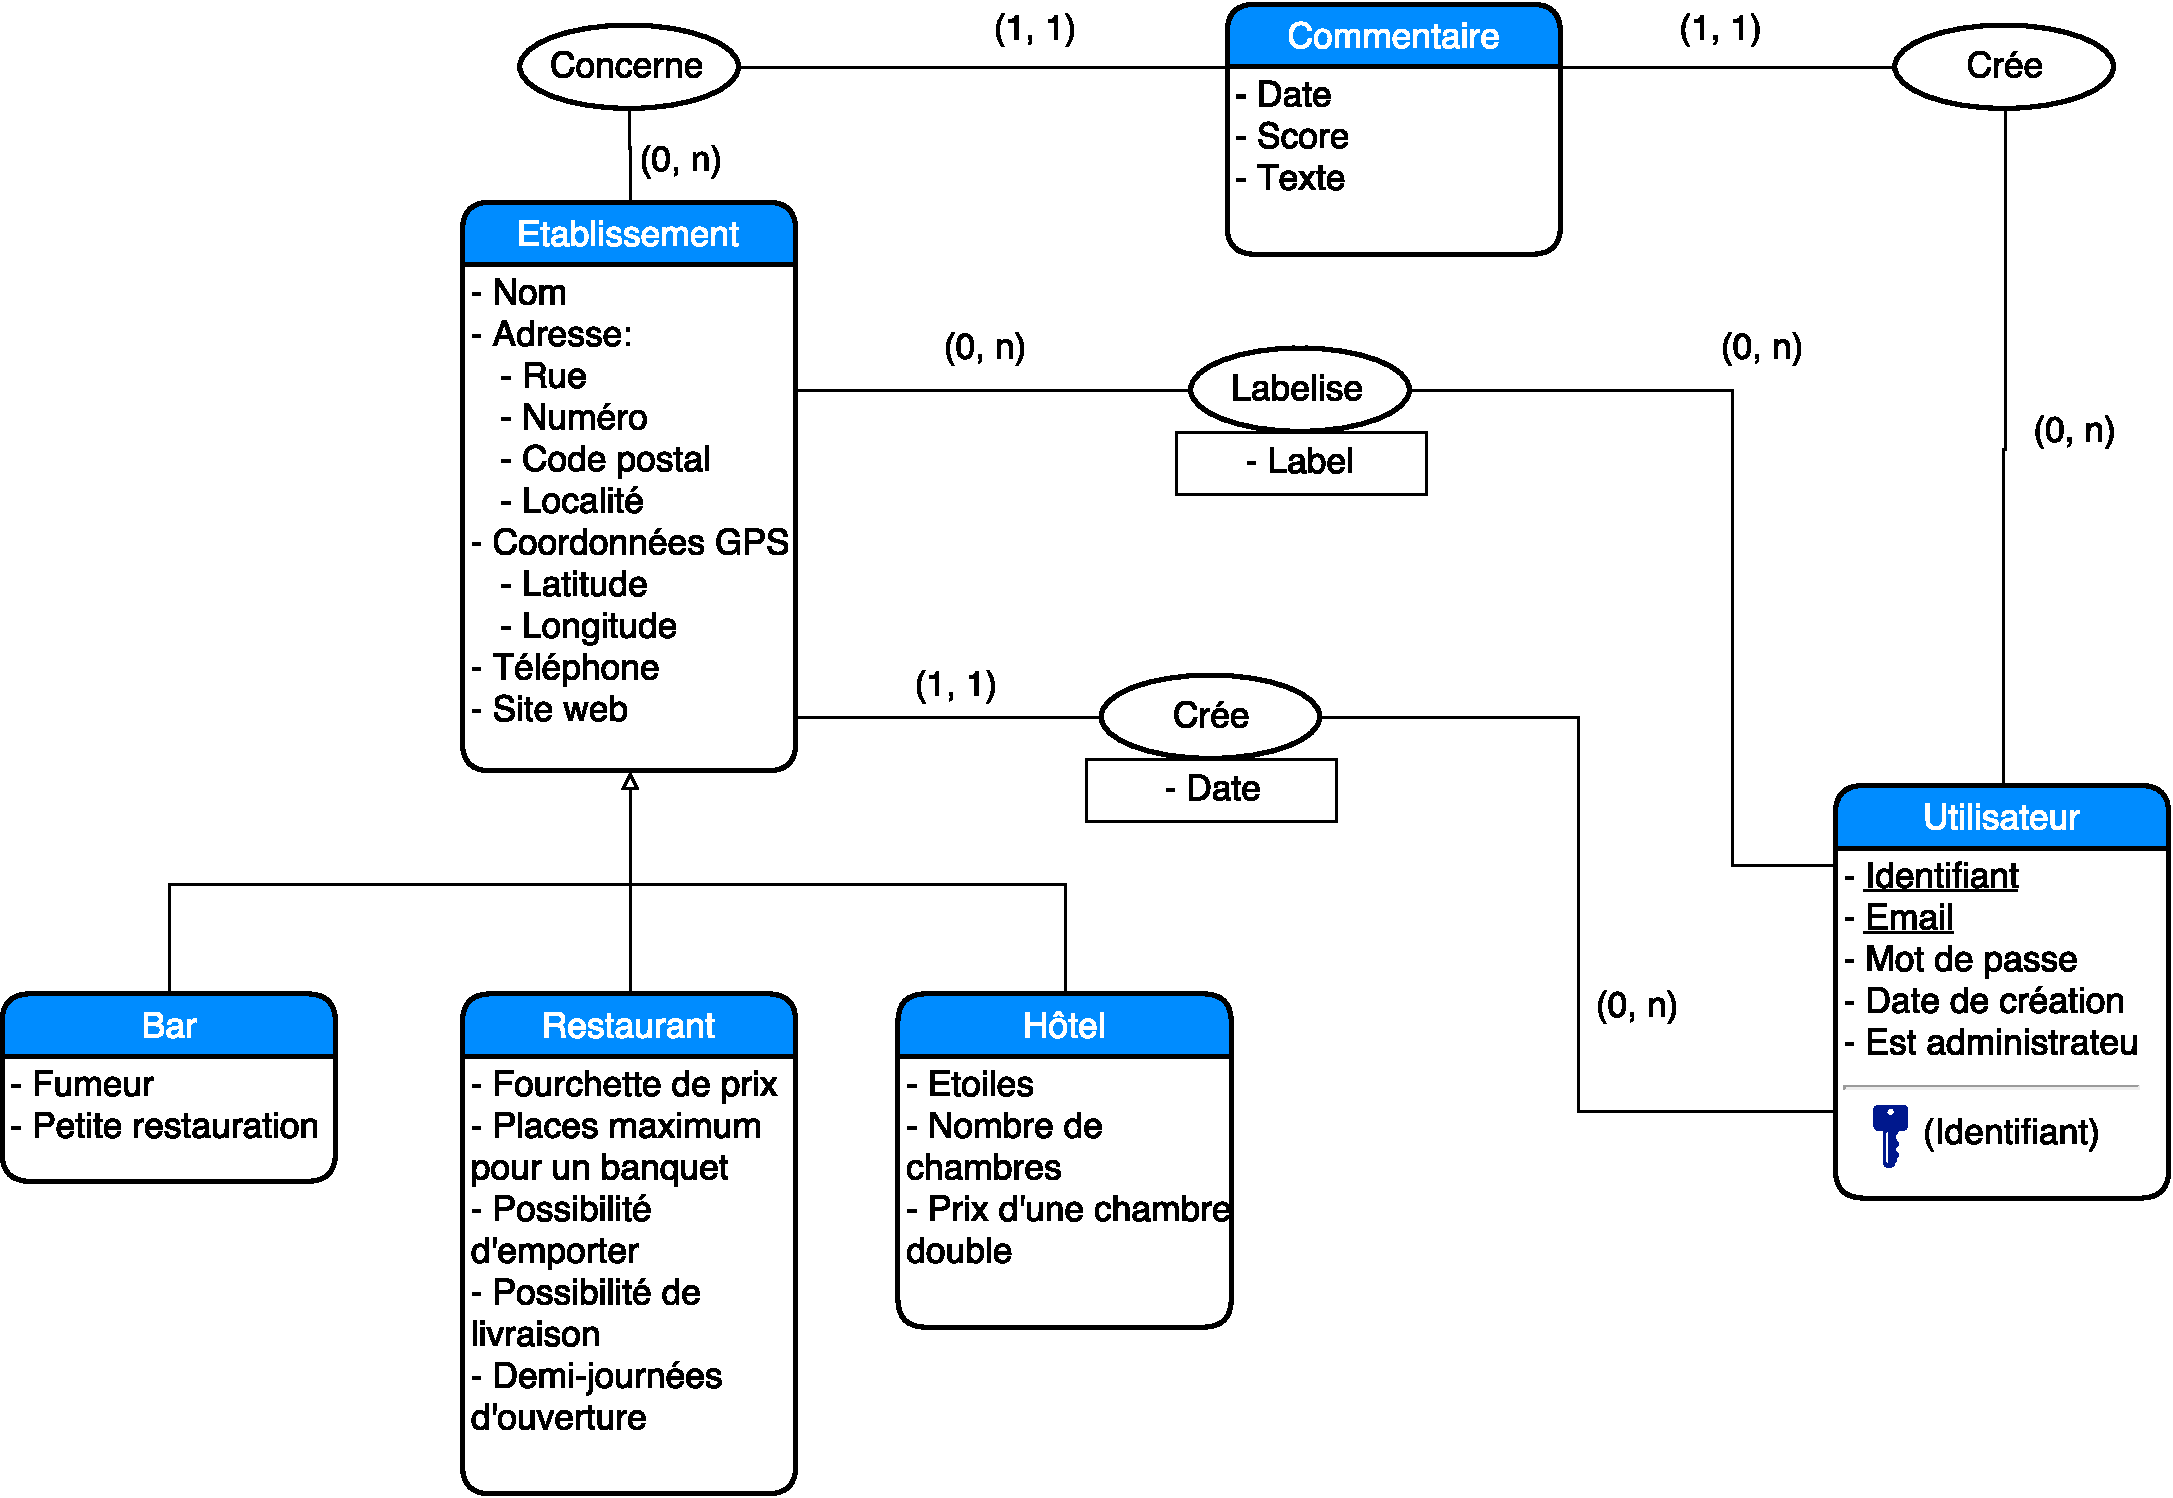
\includegraphics[scale=0.40]{EA.pdf}
    \caption{Diagramme Entité-Association}
    \label{diagram}
\end{figure}
\FloatBarrier

\subsection{Contraintes}

Les contraintes sont les suivantes :
\begin{itemize}
  \item L'\textit{UtilisateurId} d'un \textit{Etablissement} ne peut référencer qu'un \textit{Utilisateur} dont le champ \textit{EstAdministrateur} est vrai.
  \item La \textit{DateCretation} d'un \textit{Etablissement} doit être surpérieure à la \textit{DateCretation} de l'\textit{Utilisateur} qui l'a créé.
  \item La \textit{Latitude} (respectivement \textit{Longitude}) d'un \textit{Etablissement} doit appartenir à l'intervalte $[-90, 90]$ (respectivement $[-180, 180]$)
  \item Le champ \textit{Etoiles} d'un \textit{Hotel} doit appartenir à $[0,5]$
  \item Le champ \textit{Etoiles} d'un \textit{Commentaire} doit appartenir à $[0,5]$

\end{itemize}




\section{Modèle relationnel}
\subsection{Modèle}


\begin{description}
\item[Utilisateur](
    \underline{Id},
    \underline{Email},
    MotDePasse,
    DateCretaion,
    EstAdministrateur)

\item[Etablissement](
    \underline{Id},
    Type,
    Nom,
    Telephone,
    \textit{SiteWeb},
    Rue,
    Numero,
    CodePostal,
    Localite,
    Latitude,
    Longitude,
    DateCretation
    UtilisateurId)

    \begin{itemize}
        \item Etablissement.Type est une énumération de (Hotel, Bar, Restaurant)
        \item Etablissement.UtilisateurId référence Utilisateur.Id
    \end{itemize}

\item[Restaurant](
    \underline{EtablissementId},
    FourchettePrix,
    PlacesMaximum,
    Emporter,
    Livraison,
    DemiJoursOuverture)

    \begin{itemize}
        \item Restaurant.EtablissementId référence Etablissement.Id
    \end{itemize}

\item[Bar](
    \underline{EtablissementId},
    Fumeur,
    Restauration)

    \begin{itemize}
        \item Bar.EtablissementId référence Etablissement.Id
    \end{itemize}

\item[Hotel](
    \underline{EtablissementId},
    Etoiles,
    NombreChambres,
    PrixChambreDouble)

    \begin{itemize}
        \item Hotel.EtablissementId référence Etablissement.Id
    \end{itemize}

\item[Commentaire](
    \underline{Id},
    EtablissementId,
    UtilisateurId,
    Date,
    Score,
    Texte)

    \begin{itemize}
        \item Commentaire.EtablissementId référence Etablissement.Id
        \item Commentaire.UtilisateurId référence Utilisateur.Id
        \item (EtablissementId, UtilisateurId, Date) est unique
    \end{itemize}

\item[Label](
    \underline{Id},
    \underline{Nom})

\item[LabelEtablissement](
    \underline{Id},
    EtablissementId,
    UtilisateurId,
    LabelId)

    \begin{itemize}
        \item LabelEtablissement.EtablissementId référence Etablissement.Id
        \item LabelEtablissement.UtilisateurId référence Utilisateur.Id
        \item LabelEtablissement.LabelId référence Label.Id
        \item (EtablissementId, UtilisateurId, LabelId) est unique
    \end{itemize}

\end{description}

\section{Remarques}

Nous avons ajouté un champ \textit{Type} à la table \textit{Etablissement} pour pouvoir distinguer dans la table \textit{Etablissement} un bar d'un restaurant sans devoir \texttt{JOIN} sur les tables bar et restaurant. Cela nous permet par exemple de faire une requête ``Récupérer la liste des adresses des bars'' avec une simple \texttt{SELECT}.

De plus il faudra rajouter une contrainte pour que \textit{Bar.EtablissementId}, \textit{Restaurant.EtablissementId} et \textit{Hotel.EtablissementId} soient uniques, ce qui permet de garder la relation ``one-to-one'' entre \textit{Etablissement} et \textit{Bar}, \textit{Restaurant}, \textit{Hotel}.

Nous avons considéré que deux utilisateurs ne peuvent avoir la même adresse email; l'adresse email d'un \textit{Utilisateur} doit donc être unique.


\section{Sript DDL de création de la base de données}

\section{Requêtes}

\section{R1}
\subsection{AR:}
\(
BC(C_1, C_2, C_3) \leftarrow \pi_{C_1.eid, C_2.eid, C_3.eid} (((C_1 \join_{C_1.id != C_2.id \land C_1.score > 3 \land C_2.score>3} C_2)\\
\join_{C_1.id != C_3.id \land C_2.id != C3.id \land C_3.score>3}) \join_{C_1.uid = U.id \land C_2.uid = U.id \land C_3.uid = U.id}(\sigma_{U.username = "Brenda"}(U)))
\)\\

\(
AC(uid, C_1, C_2, C_3) \leftarrow \pi_{U.id, C_1.eid, C_2.eid, C_3.eid} (((C_1 \join_{C_1.id != C_2.id \land C_1.score > 3 \land C_2.score>3} C_2)\\
\join_{C_1.id != C_3.id \land C_2.id != C3.id \land C_3.score>3}) \join_{C_1.uid != U.id \land C_2.uid != U.id \land C_3.uid != U.id}(\sigma_{U.username = "Brenda"}(U)))
\)\\

\(
\pi_{AC.uid}(BC \join_{BC.C_1 = AC.C_1 \land BC.C_2 = AC.C_2 \land BC.C_3 = AC.C_3} AC)
\)

\subsection{TC}
\(
\{
u|users(u) \land \exists b(users(b) \land b.username="Brenda") \land u.id \neq b.id
\land\\
\exists e_1(etablissement(e_1) \land \exists c_1 \exists c_2(comment(c_1)\land comment(c_2) \land c_1.uid = u.id \land c_1.score > 3 \land c_2.uid = b.uid \land c_2.score >3))
\land\\
\exists e_2(etablissement(e_2) \land e_1 \neq e_2 \land \exists c_3 \exists c_4(comment(c_3)\land comment(c_4) \land c_3.uid = u.id \land c_3.score > 3 \land c_4.uid = b.uid \land c_4.score >3))
\land\\
\exists e_3(etablissement(e_3) \land e_1 \neq e_3 \land e_2 \neq e_3 \land \exists c_5 \exists c_6(comment(c_5)\land comment(c_6) \land c_5.uid = u.id \land c_5.score > 3 \land c_6.uid = b.uid \land c_6.score >3))
\}
\)

\section{R2}
\subsection{AR}
\(
AC \leftarrow \pi_{C.uid, C.eid}(\sigma_{C.score>3}(C))
\\
BC \leftarrow \pi_{C.eid}(\sigma_{U.name="Brenda", C.score>3}(C*U))
\\
U \leftarrow  \pi_{AC.uid}(AC \div BC)
\\
\pi_{C.eid}(\sigma_{C.uid = U.uid \land C.score>3}(C))
\)

\subsection{TC}
\(
\{
e|etablissement(e) \land \exists c(comment(c) \land c.score>3 \land c.eid = e.id \land \exists u(users(u) \land c.uid = u.id \land \forall f \forall b(comment(f) \land users(b) \land f.uid = b.uid\land b.username="Brenda" \land f.score > 3 \rightarrow \exists a(comment(a)\land a.uid = u.id \land f.eid = a.eid\land a.score > 3)))))
\}
\)

\section{R3}
\subsection{AR}
\(
Ew2C \leftarrow \pi_{C_1.eid, C_1.id}(C_1 \join_{C_1.eid=C_2.eid \land C_1.id != C_2.id})
\\
\pi_{E.id}(\pi_{E.id, C.id}(E \leftouterjoin_{E.id=C.eid}  C) - EW2C)
\)
\subsection{TC}

\(
\{e | etablissement(e) \land \exists c(comment(c) \land c.eid = e.id) \rightarrow \neg\exists d(comment(d) \land d.eid = e.id \land d.id \neq c.id)\}
\)

\section{R4}
\subsection{AR}
\(
\pi_{E.uid}(E) - \pi_{E.id}(E\join_{E.id = C.id \land E.uid = C.uid}C)
\)
\subsection{TC}
\(
\{e.uid|etablissement(e)\land \neg \exists c(comment(c) \land c.uid = e.uid \land c.eid = e.id)\}
\)


\section{Implémentation et choix}
\subsection{Language et bibliothèques}

Nous avons choisi d'utiliser \textbf{Python 3} ainsi que le framework \textbf{Flask} pour implémenter notre application web. Nous avons choisi \textbf{Python 3} car il est notre langage de prédilection et qu'il dispose d'un écosystème de librairies très développé.

Nous nous étions d'abord tourné vers \textbf{Django} pour le framework web car nous avons tous les deux de l'expérience avec celui-ci et qu'il est très puissant pour prototyper rapidement (gestion automatique du CRUD\footnote{CReate, Update, Delete}, validation des formulaires, gestion des utilisateurs incluse, ...) mais après avoir rapidement essayé de l'utiliser dans utiliser son \textit{ORM} (qui fait aussi \textit{query-builder}) pour suivre les consignes, nous nous somme rendus compte que nous perdions touts les avantages de \textbf{Django} tout en gardant ses inconvénients.

Nous nous sommes donc tournés vers le framework \textbf{Flask}, qui est beaucoup plus minimal et qui nous a donc laissé plus libres dans nos choix d'implémentation, celui-ci ne proposant ni d'ORM, ni de gestion des utilisateurs ni de validation de formulaires.

\end{document}

